The convolutional layers are what makes CNN's such a strong tool. In general, a convolutional layer consists of a set of learnable filters. Applying a convolutional operation on a neuron is done by using these filters to transform the input according to the filter, and output the transformed data. As mentioned earlier, CNNs can detect important patterns. The detections of these patterns are happening in these convolutional operations.\\

\noindent
These filters also called 'kernels'. Kernels are simply just small matrixes initialized with some predefined dimensions and random values. When a kernel is applied on some feature map, the kernel simply goes across all the feature-channels.\\

\noindent
Presenting this as an example, we introduce a $3$x$3$ kernel $g$ with stride $1$x$1$. The kernel will stride over all possible regions of the input, where the kernel can fit. Simply finding the dot-product between the regional values of the input $f$, and the kernel values of $g$.

$$ g = \begin{bmatrix}
-1 & 1 & 0 \\
-1 & 1 & 0 \\
-1 & 1 & 0
\end{bmatrix}
$$

\noindent
This means, that if some were to use the filter kernel $g$, on some input image. This filter $g$ would simply highlight the left vertival edges of some input; Rotating the filter, whould result in finding right vertical- and horicontal edges presented in the image, depending on how much the filter is rotated. Due to bounderies; using a filter greater than $1$x$1$ will yield a smaller output matrix. It is possible to introduce padding to avoid dimension loss.\\

\noindent
Lastly, the convolutional layers have something called stride. The stride value defines how the filter travels over the input. Meaning how many steps it takes before calculating a new dot-product. In the example given in figure(~\ref{fig:conv2} and ~\ref{fig:conv1}), we have a stride size of $1$x$1$. This means, that every single region where a $3$x$3$ can fit in the input, the dot-product will be calculated. If we were to change the stride to size $2$x$1$, the output would become smaller, since we take bigger steps, each time we are calculating the dot-product, see figure(~\ref{fig:1d_stride} and ~\ref{fig:2d_stride}).

\begin{figure}[!ht]
  \centering
  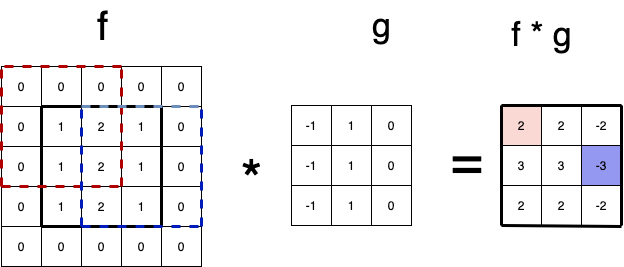
\includegraphics[scale=0.4]{latex/imgs/conv1_highVert_stride.png}
  \caption{Shows how a 3x3 left vertical edge filter acts on a 5x5 pixel feature map, with stride 1x1}\label{Baseline:before}
  \label{fig:conv2}
\end{figure}

\noindent
Given that we are looking at sequences which are one dimensional, the filtering will look like:

\begin{figure}[!ht]
  \centering
  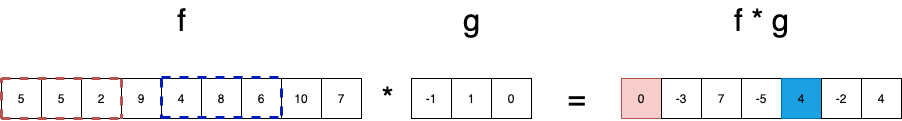
\includegraphics[scale=0.4]{latex/imgs/conv2_vert_stride.png}
  \caption{Shows how a 1x3 left vertical edge filter acts on a 1x9 feature map, with stride 1}\label{Baseline:before}
  \label{fig:conv1}
\end{figure}

\noindent
The following figures represents how the output would look like if the stride was different from 1x1.

\begin{figure}[!ht]
  \centering
  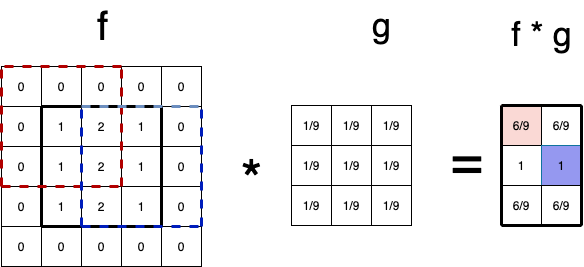
\includegraphics[scale=0.4]{latex/imgs/conv1_stride.png}
  \caption{Shows how a 3x3 mean filter acts on a 5x5 pixel feature map, with stride 2x1}\label{Baseline:before}
  \label{fig:2d_stride}
\end{figure}

\begin{figure}[!ht]
  \centering
  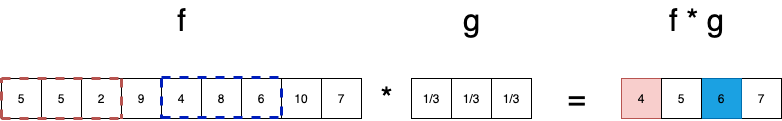
\includegraphics[scale=0.4]{latex/imgs/conv2_stride.png}
  \caption{Shows how a 1x3 mean filter acts on a 1x9 feature map, with stride 2}\label{Baseline:before}
  \label{fig:1d_stride}
\end{figure}
